\documentclass[a4paper,12pt]{article}
\usepackage[a4paper, margin=2.5cm]{geometry}
\usepackage[pdftex]{graphicx}
\usepackage{tikz}
\usepackage{pgfplots}
\usepackage{enumitem}
\usepackage{float}
\usepackage[document]{ragged2e}
\usepackage[utf8]{inputenc}
\usepackage[T1]{fontenc}
\usepackage[spanish,es-tabla]{babel}
\renewcommand{\shorthandsspanish}{}
\usepackage{xurl}
\usepackage{lipsum}
\usepackage{mwe}
\usepackage{multirow}
\usepackage{multicol}
\usepackage{siunitx}
\usepackage{listings}
\usepackage{tabularray}
\usepackage{amsmath}
\usepackage{gensymb}


\usetikzlibrary{arrows.meta,bending}
\graphicspath{ {/home/saikkopat/Documents/ESCOM/BD/Proyecto2023-2/} }

%\usepackage[none]{hyphenat}

\title{Proyecto Base de Datos}
\author{Aguilar Ibarra José Moisés \and González Cárdenas Ángel Aquilez \and Pérez Olivares José Julio}

\pgfplotsset{compat=1.18}
\begin{document}

\begin{titlepage}
	\begin{tikzpicture}[overlay, remember picture]
		\path (current page.north east) ++(-0.3,-1.5) node[below left] {
\includegraphics[width=0.35\textwidth]{/home/saikkopat/Documents/LOGOS IPN/EscudoESCOM}};
	\end{tikzpicture}
	\begin{tikzpicture}[overlay, remember picture]
		\path (current page.north west) ++(1.5,-1) node[below right] {
\includegraphics[width=0.2\textwidth]{/home/saikkopat/Documents/LOGOS IPN/logo}};
	\end{tikzpicture}
	\begin{center}
		\vspace{-1.5cm}
		{\LARGE Instituto Politécnico Nacional\par}
		\vspace{.5cm}
		{\LARGE Escuela Superior de Cómputo\par}
		\vspace{3cm}
		{\large Unidad de aprendizaje:}\\{\Large Bases de Datos\par}
		\vspace{2cm}
		{\scshape\Huge Proyecto\par}
		{\itshape\Large Clínica Odontológica\par}
		\vfill
		\vspace{.7cm}
		{\Large Grupo: 3CV1\par}
		\vspace{.7cm}
		{\Large Integrantes:\par}
		\vspace{.5cm}
		{\Large Aguilar Ibarra José Moisés\par}
		{\Large Boleta: 2022630329\par}
		\vspace{.5cm}
		{\Large González Cárdenas Ángel Aquilez\par}
		{\Large Boleta: 2016630152\par}
		\vspace{.5cm}
		{\Large Pérez Olivares José Julio\par}
		{\Large Boleta: 2022630070\par}
		\vspace{1cm}
		{\Large Profesor: Blanco Almazán Iván Eduardo\par}
		\vfill
	\end{center}
\end{titlepage} 

\newpage

\tableofcontents

\newpage

\usepgfplotslibrary{units}
\justifying

\section{Introducción}

El presente escrito documenta el proceso de resolución de una problemática particular presentada como parte del proyecto de evaluación correspondiente al semestre \emph{2023-2} de la unidad de aprendizaje \emph{Bases de Datos} para la carrera de \emph{Ingeniería en Sistemas Computacionales} del programa académico \emph{ISC2020}.

\section{Problemática a resolver}

\begin{large}Clínica odontológica\end{large}

\vspace{0.5cm}

Una nueva clínica abre sus instalaciones con la problemática de que necesita un sistema que le ayude a administrar desde sus tratamientos hasta los diversos pacientes que atiende. Para ello la clínica busca almacenar toda la información referente a los diversos pacientes que atenderá. Para ello el sistema guardará cada paciente con su nombre compuesto de nombre, apellido paterno y materno, la dirección dada por calle, número, colonia y el código postal, su fecha de nacimiento por la cual el sistema deberá calcular la edad.\par

\vspace{0.5cm}

Este paciente podrá solicitar vía telefónica una consulta por lo que se le proporcionará la fecha de consulta y el número de su consulta. Cabe aclarar que este número de consulta ayudará a saber cuál fue la consulta en el tiempo de vida de la clínica y no en el día. Cada consulta es brindada por un odontólogo, el cual el administrador registrará su nombre completo dividido en su nombre y apellidos, así como la especialidad en el área que tiene, es por ello por lo que dentro de la clínica se le dará automáticamente un número de trabajador.\par

\vspace{0.5cm}

Durante cada consulta en la cual se encuentre el odontólogo, se realizarán diversos tratamientos los cuales tienen un precio. Estos tratamientos recibirán un nombre clave, ya que son distintos para cada consulta por lo que el sistema deberá de almacenar los tratamientos mediante una fecha de inicio del tratamiento y el odontólogo podrá seleccionar la opción de terminado en caso de que el tratamiento haya finalizado, lo que arrojará la fecha de fin.\par

\vspace{0.5cm}

Debido a que esta clínica ya tenía una sucursal cercana y se planea abrir una tercera clínica, el sistema guardará el local desde donde el odontólogo trabaja apoyándose que cada local le demos un nombre característico, así como la calle, el número y la ciudad. Por parte del odontólogo, el sistema deberá registrar el día en que fue a laborar en ese local, el horario de inicio y de fin en el que se retiró del local. Esto también aplica para cuando tenga que asistir a dicho local por caso de emergencia.\par

\vspace{0.5cm}

Por último, debido a que cada clínica estará conectada al sistema del local en donde se encuentre, se debe tener un registro que pueda existir más de un consultorio en cada local por lo que necesitaremos saber en todo momento con cuantos consultorios cuenta esa clínica, así como el equipo que posee. Durante la realización de cada inventario, cada equipo se registra por su número de serie, el tipo de equipo y la última fecha en la que se le dio mantenimiento.\par

\vspace{0.5cm}

\section{Diagramas \textit{Entidad-Relación}}
\subsection{\textit{Entidad-Relación}}

Después de analizar y realizar la abstracción de la problemática, se identificaron las siguientes \emph{entidades} y sus \emph{atributos}:\\

\begin{enumerate}
	\item \textbf{Paciente}:
		\begin{enumerate}
			\item \emph{id\_paciente}
			\item nombre\_completo: nombres, apellido\_paterno, apellido\_materno
			\item dirección\_paciente: calle, número, colonia, código\_postal
			\item fecha\_nacimiento, edad
			\item teléfono
		\end{enumerate}

	\item \textbf{Consulta}:
		\begin{enumerate}
			\item \emph{id\_consulta}
			\item fecha\_consulta
		\end{enumerate}


	\item \textbf{Odontólogo}:
		\begin{enumerate}
			\item \emph{id\_empleado}
			\item nombre\_completo: nombres, apellido\_paterno, apellido\_materno
			\item especialidad
		\end{enumerate}


	\item \textbf{Tratamiento}:
		\begin{enumerate}
			\item  \emph{id\_tratamiento}
			\item nombre\_clave
			\item precio
		\end{enumerate}


	\item \textbf{Sucursal}:
		\begin{enumerate}
			\item \emph{id\_sucursal}
			\item nombre\_sucursal
			\item direccion\_sucursal: calle\_sucursal, numero\_sucursal, ciudad\_sucursal
			\item capacidad
		\end{enumerate}


	\item \textbf{Consultorio}: \emph{id\_consultorio}

	\item \textbf{Equipo}:
		\begin{enumerate}
			\item \emph{numero\_serie}
			\item descripcion
			\item fecha\_mantenimiento
		\end{enumerate}

\end{enumerate}

\newpage

Y para las \emph{relaciones} se identificaron las siguientes:

\begin{enumerate}
	\item Paciente - Consulta (1:N) 
	\item Consulta - Odontólogo (N:1)
	\item Consulta - Tratamiento (1:N)
	\item Odontólogo - Sucursal (N:M)
	\item Sucursal - Consultorio (1:N)
	\item Consultorio - Equipo (1:N)
\end{enumerate}


De modo que gráficamente, se visualiza de la siguiente forma:\\

\begin{figure}[!h]
\centering
	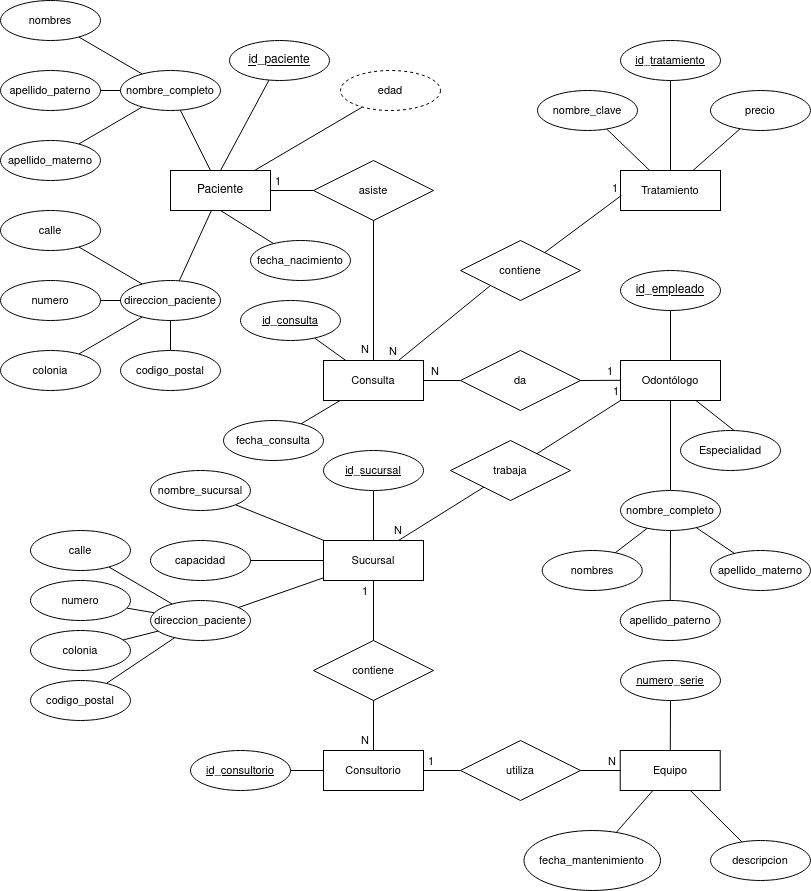
\includegraphics[width=.85\textwidth]{ER}
	 \caption{Diagrama Entidad-Relación}
\end{figure}

\subsection{\textit{Entidad-Relación Extendido}}

Para este apartado, extendemos el caso que la problemática plantea como \emph{emergencia}, considerándose como un tipo de \textit{consulta}. \\

Por otra parte, se agrega la entidad \emph{cita} para denotar a los contactos telefónicos que realizan los pacientes previos a la consulta.\\

Así, se visualiza de la siguiente forma:\\

\begin{figure}[!h]
\centering
	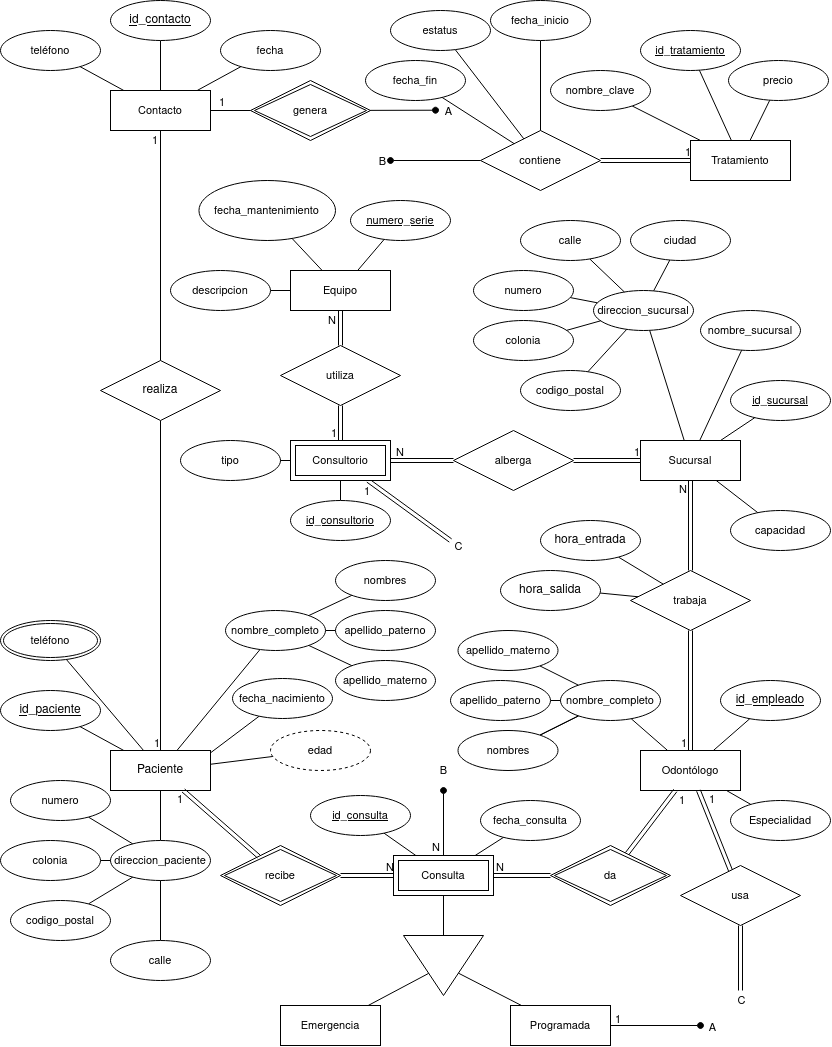
\includegraphics[width=.85\textwidth]{ERE}
	 \caption{Diagrama Entidad-Relación}
\end{figure}


\section{Diagrama Relacional}
Del diagrama anterior se generó el diagrama relacional:

\begin{figure}[!h]
\centering
	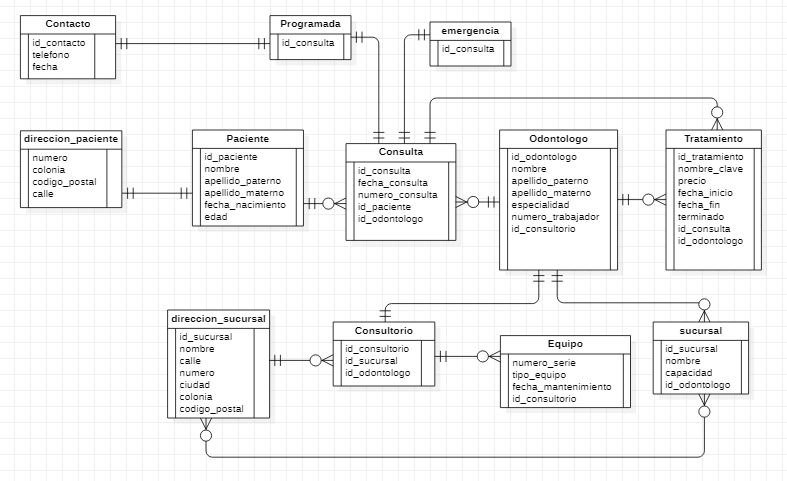
\includegraphics[width=.85\textwidth]{REL}
	 \caption{Diagrama Entidad-Relación}
\end{figure}

\newpage

\section{Diccionario de datos}

De los anteriores diagramas se utilizaron los siguientes tipos de datos para su implementación en el sistema gestor de base de datos que alberga la base de datos:\\

\textbf{Paciente} \\ \emph{Objetivo}: La tabla \emph{paciente} alberga información relevante sobre los pacientes que acuden a la clínica odontológica.
\begin{enumerate}
	\item \underline{id\_paciente} \textbf{Llave primaria}, entero, \emph{no nulo}, \textit{auto-incrementable}
	\item \texttt{nombre\_paciente} texto, \emph{no nulo}
	\item \texttt{apellido\_paterno} texto, \emph{no nulo}
	\item \texttt{apellido\_materno} texto, \emph{no nulo}
	\item \texttt{fecha\_nacimiento} fecha, \emph{no nulo}
	\item \texttt{edad} entero, \emph{no nulo}
\end{enumerate}

\emph{Creación de la tabla con SQL}: 
\begin{verbatim}
CREATE TABLE if not exists Paciente (
  id_paciente INT PRIMARY KEY AUTO_INCREMENT,
  nombre_paciente VARCHAR(50) NOT NULL,
  apellido_paterno VARCHAR(50) NOT NULL,
  apellido_materno VARCHAR(50) NOT NULL,
  fecha_nacimiento DATE NOT NULL,
  edad INT NOT NULL
);
\end{verbatim}

\emph{Stored procedures}:

\begin{verbatim}
REATE PROCEDURE sp_InsertarPaciente(
    IN nombre VARCHAR(50),
    IN apellido_paterno VARCHAR(50),
    IN apellido_materno VARCHAR(50),
    IN fecha_nacimiento DATE,
    IN edad INT,
    IN calle VARCHAR(100),
    IN numero INT,
    IN colonia VARCHAR(100),
    IN codigo_postal INT
)
BEGIN
    INSERT INTO Paciente (nombre_paciente, apellido_paterno, apellido_materno, fecha_nacimiento, edad)
    VALUES (nombre, apellido_paterno, apellido_materno, fecha_nacimiento, edad);
    
    SET @id_paciente = LAST_INSERT_ID();
    
    INSERT INTO direc_paciente (calle, numero, colonia, codigo_postal, id_paciente)
    VALUES (calle, numero, colonia, codigo_postal, @id_paciente);
END
\end{verbatim}


\textbf{direc\_paciente} \\ \emph{Objetivo}: Alberga las direcciones de los pacientes y se relaciona con el paciente asociado mediante una llave foránea.
\begin{enumerate}
	\item \underline{id\_paciente} \textbf{Llave foránea}
	\item \texttt{calle} texto, \emph{no nulo}
	\item \texttt{numero} entero, \emph{no nulo}
	\item \texttt{colonia} texto, \emph{no nulo}
	\item \texttt{codigo\_postal} fecha, \emph{no nulo}
\end{enumerate}

\emph{Creación de la tabla con SQL}: 
\begin{verbatim}
CREATE TABLE if not exists direc_paciente (
  calle VARCHAR(100) NOT NULL,
  numero INT NOT NULL,
  colonia VARCHAR(100) NOT NULL,
  codigo_postal INT NOT NULL,
  id_paciente INT NOT NULL,
  FOREIGN KEY (id_paciente) REFERENCES Paciente(id_paciente)
);
\end{verbatim}

\emph{Triggers}: 

\begin{verbatim}
CREATE TRIGGER tr_direc_paciente_delete
BEFORE DELETE ON direc_paciente
FOR EACH ROW
BEGIN
    DELETE FROM direc_paciente WHERE id_paciente = OLD.id_paciente;
END
\end{verbatim}


\textbf{Odontologo} \\ \emph{Objetivo}: Alberga información de control sobre los odontólogos.
\begin{enumerate}
	\item \underline{numero\_empleado} \textbf{Llave primaria}, entero, \emph{no nulo}, \textit{auto-incrementable}
	\item \texttt{nombre} texto, \emph{no nulo}
	\item \texttt{apellido\_paterno} texto, \emph{no nulo}
	\item \texttt{apellido\_materno} texto, \emph{no nulo}
	\item \texttt{especialidad} texto, \emph{no nulo}
\end{enumerate}

\emph{Creación de la tabla con SQL}: 
\begin{verbatim}
CREATE TABLE if not exists Odontologo (
  id_odontologo INT PRIMARY KEY AUTO_INCREMENT,
  nombre VARCHAR(50) NOT NULL,
  apellido_paterno VARCHAR(50) NOT NULL,
  apellido_materno VARCHAR(50) NOT NULL,
  especialidad VARCHAR(100) NOT NULL,
  numero_trabajador INT NOT NULL,
  id_consultorio INT NOT NULL
);

ALTER TABLE Odontologo ADD FOREIGN KEY (id_consultorio) REFERENCES Consultorio(id_consultorio);
\end{verbatim}

\emph{Triggers}: 

\begin{verbatim}
CREATE TRIGGER tr_Odontologo_delete
BEFORE DELETE ON Odontologo
FOR EACH ROW
BEGIN
    DELETE FROM Odontologo WHERE id_consultorio = OLD.id_consultorio;
END
\end{verbatim}

\emph{Stored procedures}: Actualiza la especialidad de un odontólogo.

\begin{verbatim}
CREATE PROCEDURE sp_ActualizarEspecialidad(
    IN odontologo_id INT,
    IN nueva_especialidad VARCHAR(100)
)
BEGIN
    UPDATE Odontologo
    SET especialidad = nueva_especialidad
    WHERE id_odontologo = odontologo_id;
END
\end{verbatim}


\textbf{Consulta} \\ \emph{Objetivo}: Conjunta la información sobre los pacientes que reciben algún tratamiento, son atendidos por algún odontólogo en una hora y lugar establecidos.
\begin{enumerate}
	\item \underline{id\_consulta} \textbf{Llave primaria}, entero, \emph{no nulo}, \textit{auto-incrementable}
	\item \texttt{fecha\_consulta} fecha, \emph{no nulo}
	\item \texttt{id\_paciente} \textbf{Llave foránea}
	\item \texttt{numero\_empleado} \textbf{Llave foránea}
\end{enumerate}

\emph{Creación de la tabla con SQL}: 
\begin{verbatim}
CREATE TABLE if not exists Consulta (
  id_consulta INT PRIMARY KEY AUTO_INCREMENT,
  fecha_consulta DATE NOT NULL,
  numero_consulta INT NOT NULL,
  id_paciente INT NOT NULL,
  id_odontologo INT NOT NULL,
  FOREIGN KEY (id_paciente) REFERENCES Paciente(id_paciente),
  FOREIGN KEY (id_odontologo) REFERENCES Odontologo(id_odontologo)
);
\end{verbatim}

\emph{Triggers}: 

\begin{verbatim}
CREATE TRIGGER tr_Consulta_delete
BEFORE DELETE ON Consulta
FOR EACH ROW
BEGIN
    DELETE FROM Consulta WHERE id_paciente = OLD.id_paciente;
    DELETE FROM Consulta WHERE id_odontologo = OLD.id_odontologo;
END
\end{verbatim}

\emph{Stored procedure}: Obtiene la lista de consultas de un paciente

\begin{verbatim}
CREATE PROCEDURE sp_ConsultasPorPaciente(
    IN paciente_id INT
)
BEGIN
    SELECT *
    FROM Consulta
    WHERE id_paciente = paciente_id;
END
\end{verbatim}

\textbf{Tratamiento} \\ \emph{Objetivo}: Contiene información sobre los tratamientos, costos, duración y estatus del mismo.
\begin{enumerate}
	\item \underline{id\_tratamiento} \textbf{Llave primaria}, entero, \emph{no nulo}, \textit{auto-incrementable}
	\item \texttt{nombre\_clave} texto, \emph{no nulo}
	\item \texttt{precio} flotante, \emph{no nulo}
\end{enumerate}

\emph{Creación de la tabla con SQL}: 
\begin{verbatim}
CREATE TABLE if not exists Tratamiento (
  id_tratamiento INT PRIMARY KEY AUTO_INCREMENT,
  nombre_clave VARCHAR(100) NOT NULL,
  precio DECIMAL(10,2) NOT NULL,
  fecha_inicio DATE NOT NULL,
  fecha_fin DATE,
  terminado BOOLEAN NOT NULL,
  id_consulta INT NOT NULL,
  id_odontologo INT NOT NULL,
  FOREIGN KEY (id_consulta) REFERENCES Consulta(id_consulta),
  FOREIGN KEY (id_odontologo) REFERENCES Odontologo(id_odontologo)
);
\end{verbatim}

\emph{Triggers}: 

\begin{verbatim}
CREATE TRIGGER tr_Tratamiento_delete
BEFORE DELETE ON Tratamiento
FOR EACH ROW
BEGIN
    DELETE FROM Tratamiento WHERE id_consulta = OLD.id_consulta;
    DELETE FROM Tratamiento WHERE id_odontologo = OLD.id_odontologo;
END
\end{verbatim}


\textbf{Sucursal} \\ \emph{Objetivo}: Conjuntar la información de las diferentes sucursales de la clínica, que contiene consultorios y equipo de forma indirecta. Capacidad hace referencia al número de consultorios que puede albergar.
\begin{enumerate}
	\item \underline{id\_sucursal} \textbf{Llave primaria}, entero, \emph{no nulo}, \textit{auto-incrementable}
	\item \texttt{nombre\_sucursal} texto, \emph{no nulo}
	\item \texttt{capacidad} entero, \emph{no nulo}
\end{enumerate}

\emph{Creación de la tabla con SQL}: 
\begin{verbatim}
CREATE TABLE if not exists sucursal (
  id_sucursal INT PRIMARY KEY AUTO_INCREMENT,
  nombre_sucursal VARCHAR(100) NOT NULL,
  capacidad_sucursal INT NOT NULL,
  id_odontologo INT NOT NULL,
  FOREIGN KEY (id_odontologo) REFERENCES Odontologo(id_odontologo)
);
\end{verbatim}

\emph{Triggers}:

\begin{verbatim}
CREATE TRIGGER tr_sucursal_delete
BEFORE DELETE ON sucursal
FOR EACH ROW
BEGIN
    DELETE FROM sucursal WHERE id_odontologo = OLD.id_odontologo;
END
\end{verbatim}

\textbf{direc\_sucursal} \\ \emph{Objetivo}: Alberga las direcciones de las sucursales.
\begin{enumerate}
	\item \underline{id\_sucursal} \textbf{Llave foránea}
	\item \texttt{calle} texto, \emph{no nulo}
	\item \texttt{numero} entero, \emph{no nulo}
	\item \texttt{colonia} texto, \emph{no nulo}
	\item \texttt{ciudad} texto, \emph{no nulo}
	\item \texttt{codigo\_postal} fecha, \emph{no nulo}
\end{enumerate}

\emph{Creación de la tabla con SQL}: 
\begin{verbatim}
CREATE TABLE if not exists direc_sucursal (
  id_sucursal INT NOT NULL,
  calle_sucursal VARCHAR(100) NOT NULL,
  numero_sucursal INT NOT NULL,
  colonia_sucursal VARCHAR(100) NOT NULL,
  ciudad_sucursal VARCHAR(100) NOT NULL,
  codigoPostal_sucursal INT NOT NULL,
  FOREIGN KEY (id_sucursal) REFERENCES sucursal(id_sucursal)
);
\end{verbatim}

\emph{Triggers}: 

\begin{verbatim}
CREATE TRIGGER tr_direc_sucursal_delete
BEFORE DELETE ON direc_sucursal
FOR EACH ROW
BEGIN
    DELETE FROM direc_sucursal WHERE id_sucursal = OLD.id_sucursal;
END
\end{verbatim}


\textbf{Consultorio} \\ \emph{Objetivo}: Alberga información sobre los diferentes consultorios que se utilizan en la clínica así como el odontólogo asignado.
\begin{enumerate}
	\item \underline{id\_consultorio} \textbf{Llave primaria}, entero, \emph{no nulo}, \textit{auto-incrementable}
	\item \underline{id\_sucursal} \textbf{Llave foránea}
	\item \underline{numero\_empleado} \textbf{Llave foránea}
\end{enumerate}

\emph{Creación de la tabla con SQL}: 
\begin{verbatim}
CREATE TABLE if not exists Consultorio (
  id_consultorio INT PRIMARY KEY AUTO_INCREMENT,
  id_sucursal INT NOT NULL,
  id_odontologo INT NOT NULL,
  FOREIGN KEY (id_sucursal) REFERENCES sucursal(id_sucursal),
  FOREIGN KEY (id_odontologo) REFERENCES Odontologo(id_odontologo)
);
\end{verbatim}

\emph{Triggers}:

\begin{verbatim}
CREATE TRIGGER tr_Consultorio_delete
BEFORE DELETE ON Consultorio
FOR EACH ROW
BEGIN
    DELETE FROM Consultorio WHERE id_sucursal = OLD.id_sucursal;
    DELETE FROM Consultorio WHERE id_odontologo = OLD.id_odontologo;
END
\end{verbatim}

\textbf{Equipo} \\ \emph{Objetivo}: Alberga información sobre el equipo que se utiliza en los consultorios.
\begin{enumerate}
	\item \underline{numero\_serie} \textbf{Llave primaria}, entero, \emph{no nulo}, \textit{auto-incrementable}
	\item \texttt{tipo\_equipo} texto, \emph{no nulo}
	\item \texttt{fecha\_mantenimiento} fecha, \emph{no nulo}
	\item \underline{id\_consultorio} \textbf{Llave foránea}
\end{enumerate}

\emph{Creación de la tabla con SQL}: 
\begin{verbatim}
CREATE TABLE if not exists Equipo (
  numero_serie VARCHAR(50) PRIMARY KEY NOT NULL,
  tipo_equipo VARCHAR(100) NOT NULL,
  fecha_mantenimiento DATE NOT NULL,
  id_consultorio INT NOT NULL,
  FOREIGN KEY (id_consultorio) REFERENCES Consultorio(id_consultorio)
);
\end{verbatim}

\emph{Triggers}:

\begin{verbatim}
CREATE TRIGGER tr_Equipo_delete
BEFORE DELETE ON Equipo
FOR EACH ROW
BEGIN
    DELETE FROM Equipo WHERE id_consultorio = OLD.id_consultorio;
END
\end{verbatim}



\textbf{Contacto} \\ \emph{Objetivo}: Debido a que los clientes pueden llamar para agendar una cita, existe esta tabla para albergar información sobre los contactos de los pacientes que terminen en una cita programada.
\begin{enumerate}
	\item \underline{id\_contacto} \textbf{Llave primaria}, entero, \emph{no nulo}, \textit{auto-incrementable}
	\item \texttt{fecha\_contacto} fecha, \emph{no nulo}
\end{enumerate}

\emph{Creación de la tabla con SQL}: 
\begin{verbatim}
CREATE TABLE if not exists Contacto (
	id_contacto INT NOT NULL PRIMARY KEY AUTO_INCREMENT
);
\end{verbatim}

\textbf{Cita programada} \\ \emph{Objetivo}: Una cita programada tiene identificación del paciente y una fecha a futuro. Enlaza el contacto del que se generó y la cita en la que terminó.
\begin{enumerate}
	\item \underline{id\_contacto} \textbf{Llave foránea}
	\item \underline{id\_consulta} \textbf{Llave foránea}
\end{enumerate}

\emph{Creación de la tabla con SQL}: 
\begin{verbatim}
CREATE TABLE if not exists Programada (
	id_consulta INT NOT NULL,
	id_contacto INT NOT NULL,
	FOREIGN KEY (id_consulta) REFERENCES Consulta(id_consulta),
	FOREIGN KEY (id_contacto) REFERENCES Contacto(id_contacto)
);
\end{verbatim}

\emph{Triggers}: 

\begin{verbatim}
CREATE TRIGGER tr_Programada_delete
BEFORE DELETE ON Programada
FOR EACH ROW
BEGIN
    DELETE FROM Programada WHERE id_consulta = OLD.id_consulta;
    DELETE FROM Programada WHERE id_contacto = OLD.id_contacto;
END
\end{verbatim}


\textbf{Emergencia} \\ \emph{Objetivo}: Similar al anterior, pero con el carácter de emergencia.
\begin{enumerate}
	\item \underline{id\_contacto} \textbf{Llave foránea}
	\item \underline{id\_consulta} \textbf{Llave foránea}
\end{enumerate}

\emph{Creación de la tabla con SQL}: 
\begin{verbatim}
CREATE TABLE if not exists Emergencia (
	id_consulta INT NOT NULL,
	id_contacto INT NOT NULL,
	FOREIGN KEY (id_consulta) REFERENCES Consulta(id_consulta),
	FOREIGN KEY (id_contacto) REFERENCES Contacto(id_contacto)
);
\end{verbatim}

\emph{Triggers}: 

\begin{verbatim}
CREATE TRIGGER tr_Emergencia_delete
BEFORE DELETE ON Emergencia
FOR EACH ROW
BEGIN
    DELETE FROM Emergencia WHERE id_consulta = OLD.id_consulta;
    DELETE FROM Emergencia WHERE id_contacto = OLD.id_contacto;
END
\end{verbatim}

\section{Anexos}
\subsection{Creación de la base de datos}
Se anexa el script mediante el cual se generó la base de datos, sus respectivas inserciones y los diferentes \textit{triggers} y \textit{stored procedures} que la acompañan.\\

\newpage

\subsection{Consultas SQL}

Los siguientes enunciados describen ejercicios prácticos que se anexan como parte de la evaluación al proyecto:\\

\begin{enumerate}
	\item Genere una vista donde visualice que odontólogo atiende a que paciente.
	\item Genere un reporte donde se recupere que tratamiento realiza cada odontólogo.
	\item En que clínica trabaja que odontólogos 
	\item Genere una función que a partir de introducir el nombre completo del paciente genere lo siguiente:
Nombre\_completo\_Paciente, Edad, Tratamiento, Precio Nombre\_completo, Odontologo, Cedula Clinica
	\item Ingrese la siguiente información: Juan Ramirez Iñiguez de 38 años, ingreso a la clínica dentalink para un tratamiento de carillas, el cual tiene un costo de \$500.00, para ello el odontólogo que lo atiende se llama Maria Angeles Peña con especialidad en ortodoncia. 
	\item Genere una función que me regrese los tratamientos que ha realizado un odontólogo a partir de su nombre y de la fecha de inicio.
	\item Ingrese 10 nuevos odontólogos con información en todos los campos
	\item Ingrese 10 nuevos clientes con sus tratamientos y asígnelos a los nuevos odontólogos que ingreso. Mínimo debe estar asignado a 4 de los nuevos odontólogos.
\end{enumerate}







\end{document}